\documentclass{article}

\usepackage[T1]{fontenc} 
\usepackage[utf8]{inputenc}
\usepackage{graphicx}
\graphicspath{{./img/}}
\usepackage{amsmath, amssymb}
\usepackage[left=3cm,right=3cm,top=2cm,bottom=2cm]{geometry}
\usepackage{url}
\usepackage[linktocpage=true, hidelinks]{hyperref}
\hypersetup{
    colorlinks = true,
    linkcolor = blue
}
\usepackage{subfig}
\usepackage{float}
\usepackage[french]{babel}

\title{Rapport de Projet : Tower Defense}
\author{Youri CHANCRIN, Théo DESCOMPS, Samuel KHALIFA, Jean-Baptiste MARTINEZ}
\date{\today}

\makeatletter
\let\mytitle\@title
\let\myauthor\@author
\makeatother

\begin{document}

\begin{flushleft}

\thispagestyle{empty}

\includegraphics[width=0.2\textwidth]{enseirb-matmeca}
\graphicspath{{./img/}}

\vspace{\stretch{0.4}}

\hrulefill \\[2em]
\begin{center}
\textbf{\Huge \mytitle}\\[0.8em]
{\large equipe : projetss6-tower-19048}
\\[0.8em]
\end{center}
\hrulefill

\vspace{\stretch{0.6}}

{\large \textbf{Auteurs :} \myauthor}\\
\vspace{\stretch{0.2}}
{\large \textbf{Responsable de projet :} David Renault}\\
\vspace{\stretch{0.2}}
{\large \textbf{Enseignant référent :} Frédéric Herbreteau}

\vspace{\stretch{1}}

\begin{center}
  Première année, filière informatique\\
  Date : \today
\end{center}

\vspace{\stretch{1}}

\hfill Version actuelle du document : draft

\end{flushleft}

\newpage

\tableofcontents

\newpage

\section{Sujet}
L'objectif de ce projet est la réalisation d'un jeu de type \hyperlink{https://fr.wikipedia.org/wiki/Tower_defense}{tower defense}.

Ce genre peut se résumer en une seule phrase :
\begin{center}
    \emph{Des attaquants envahissent une zone défendue par des défenseurs.}\label{sec:description jeu}
\end{center}

\subsection{Contraintes}

La programmation fonctionnelle est le paradigme mis en avant.
Nous évitons donc au maximum la programmation impérative ou encore la programmation orienté objet.
L'exécutable est réalisé en Typescript, une surcouche de JavaScript que nous utilisons pour typer le contenu de notre programme.

\subsection{Theme}
Nous avons choisi de créer un jeu de tower defense autour du thème
du Pastafarisme, en faisant attention à éviter toute forme de violence.
Selon cette religion, la température de la Terre est inversement proportionnelle 
au nombre de pirates qu'elle contient.
Cette problématique est ajourd'hui d'une importance majeure, et nous voulons sensibiliser des joueurs aux causes climatiques.
L'objectif du jeu est donc de répandre le Pastafarisme, prêché par des pirates qui correspondent aux défenseurs de notre jeu, et de défendre le Monstre Spaghetti Volant, notre sauveur. 

\section{Conception}\label{sec:conception}

Notre description du jeu, en \hyperref[sec:description jeu]{partie \ref{sec:description jeu} }, nous permet d'en tirer les éléments fondamentaux.

Parmis ces éléments se trouvent les entités, comme les attaquants, mais aussi les défenseurs. Bien qu'elles soient antagonistes, ces entités ont des similarités, notamment dans le traitement de leurs actions. 

Nous décidons donc de les regrouper sous un même nom, les \textbf{acteurs}.


\subsection{Entité Acteur}


Les acteurs forment un ensemble d'entités aux comportements et états variés, 
qui intéragissent entre elles.

Le type acteur est très générique et peut représenter beaucoup de choses.
Pour garder une consistence entre nos acteurs, on définit des archétypes.

\begin{itemize}
   \item Spaghetti Monster : Le gentil monstre spaghetti que les défenseurs doivent protéger.
   \item Good Guy : Les défenseurs.
   \item Ignorant : Un type d'attaquant.
   \item Ignorance Spreader : Un autre type d'attaquant.
   \item Spawner : Un point d'apparition pour les attaquants.
   \item Ground : Un bout de chemin sur lequel les attaquants se déplacent.
\end{itemize}

Les types Good Guy, Ignorant et Ignorance Spreader représentent 
les défenseurs et les attaquants. Ils découlent directement de la description du jeu.
Cependant, nos acteurs comportent aussi un type Spawner et Ground.
Ces types ne peuvent ni attaquer ni être attaqués, mais ils peuvent interagir avec le reste des entités, ce qui justifie qu'ils
soient aussi considérés comme des acteurs.

En effet, Spawner peut être vu comme un attaquant immortel, et Ground 
un défenseur qui contraint le déplacement des attaquants.

Passons aux interactions entre entités.

Chaque acteur a besoin de disposer d'un ensemble de comportements qui puisse évoluer 
au cours de la partie, comme pour simuler des effets incapacitants 
ou stimulants.

Pour que ces interactions prennent effet, nos entités ont 
égalements besoin d'un état interne.

Les états internes des entités comportent toujours :

\begin{itemize}
    \item Une \textbf{position}
    \item Un \textbf{type} d'entité
\end{itemize}

Avec la diversification des acteurs vient le problème de la spécialisation qui se traduit par l'ajout d'attributs \emph{spécifiques} à chaque acteur.

Par exemple, les acteurs béligérants ont besoins d'attributs spécifiques tels que des points de croyance et une limite que ces points peuvent atteindre.

On pourrait rajouter tous les attributs nécessaires à tous les comportements 
à tous les acteurs. Mais c'est une mauvaise idée pour deux raisons.
Premièrement, cela entraînerait une modification sur le type acteur à chaque nouvel attribut ajouté, et entraînerai une modification de la signatures de certaines fonctions auxiliaires comme le constructeur.
Secondement, le type acteur aurait toujours plus d'états possibles, 
et deviendrait de plus en plus complexe et lourd à comprendre et gérer.

Pour éviter ces désagréments, nous avons séparé la responsabilité des attributs 
dépendants de certains comportements dans un champs \textbf{externalProps}.
Pour que ce champs puisse satisfaire toutes les possibilités d'attributs, il
est de type dictionnaire de quelconque. Toutefois, ce typage faible est compensé 
par la présence de fonctions getter et setter agissants comme une interface 
avec \textbf{externalProps}.

Nos acteurs sont donc parés à toute éventalité d'évolution.
Cependant, bien qu'ils disposent de comportements pouvant évoluer, ils ne peuvent modifier leurs 
états internes directement.
Nous avons besoin de quelque chose d'ordre supérieur pour gérer leurs interactions.
Quelque chose comme un système de phase.

\subsection{Système de phase}

Nos acteurs effectuent des actions qui ont des conséquences.
Cela implique qu'il y a un avant et un après aux actions.
Pour chaque type d'action, on créer une phase.
Elle agit comme un ordonnanceur. Elle obtient les intentions de chaque 
acteur pour l'action qu'elle traite, et applique les modifications, 
créant une nouvelle liste d'acteur.

Nommons un tour de jeu comme une execution de l'ensemble de nos phases.

Au cours d'un tour de jeu, les phases doivent permettre aux acteurs de réaliser les actions suivantes :
\vspace{-10px}
\begin{itemize}
  \item Se déplacer
  \item Attaquer un autre acteur
  \item Soigner un autre acteur
  \item Faire apparaitre des nouveaux acteurs
  \item Se retirer du jeu
\end{itemize}  

Dans un soucis de cohérence et d'équité entre les acteurs, 
leurs intentions sont traitées de manière synchronisées au cours des phases.
Si ce n'était pas le cas, l'ordre dans lequel les acteurs jouent pourrait influer 
sur le résultat du tour de jeu. Par exemple, si un acteur joue dans sa 
phase d'attaque, inflige des dégats à un ennemi, puis joue sa phase de déplacements,
s'eloignant et privant l'ennemi d'une juste riposte.

Le découpage d'un tour de jeu en une liste de phase permet d'être modulaire.
Il en résulte qu'il est très simple de rajouter des phases de jeu, ou de 
changer l'ordre dans lequel les acteurs agissent.

Enfin, il peut arriver que les intentions des acteurs soient incompatibles.
Par exemple, si deux acteurs ayant des collisions veulent aller au même endroit.
Chaque phase doit pouvoir résoudre les conflits qu'elle génère.

Nous disposons donc d'acteurs, qui peuvent désormais intéragir entre eux avec 
une grande modularité.

Il ne nous manque plus qu'une seule notion issue de notre description du jeu 
\ref{sec:description jeu} , celle de zone.

On aimerait contraindre nos acteurs à rester dans celle-ci. Cela 
rejoint l'idée précédente de limiter certaines actions des acteurs, en l'occurence, 
on veut interdire les acteurs de quitter notre zone de jeu.

Mais cela n'est pas possible avec nos phases, car elles n'ont justement pas 
cette notion de zone.
On va donc remédier au problème en créant un objet supérieur, un objet représentant 
un monde.

\subsection{Monde}

Notre monde doit représenter une zone de jeu.
C'est un ensemble de coordonnées sur lesquelles nos entités peuvent exister.

Grâce à lui, on va réaliser deux opérations supérieur aux phases et aux acteurs que 
l'on ne pourrait faire autrement.
Tout d'abord, contraindre tous les acteurs à se trouver dans notre monde.
Ensuite, au début de la partie, on va pouvoir définir le chemin que 
les attaquants vont parcourir lors de leur invasion sur la zone de jeu.

Avec ces trois élements que sont les acteurs, les phases et le monde, on va pouvoir 
créer des acteurs de différents types, effectuant diverses actions, le tout dans une 
zone définie.

On s'attend à un résultat de ce type \ref{fig:affichages}.

\begin{figure}[H]
    \centering
    \subfloat[][\centering Monde de taille 10 x 10.\label{fig:subfig1}]{{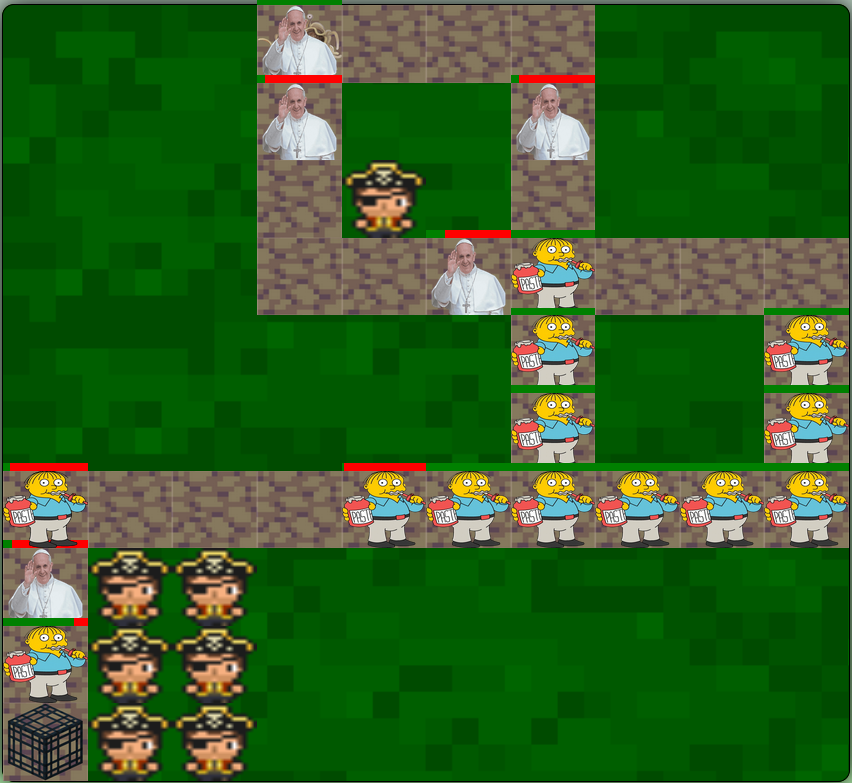
\includegraphics[height=6cm]{pastafarist_10.png} }}
    \qquad
    \subfloat[][\centering Monde de taille 20 x 20.\label{fig:subfig2}]{{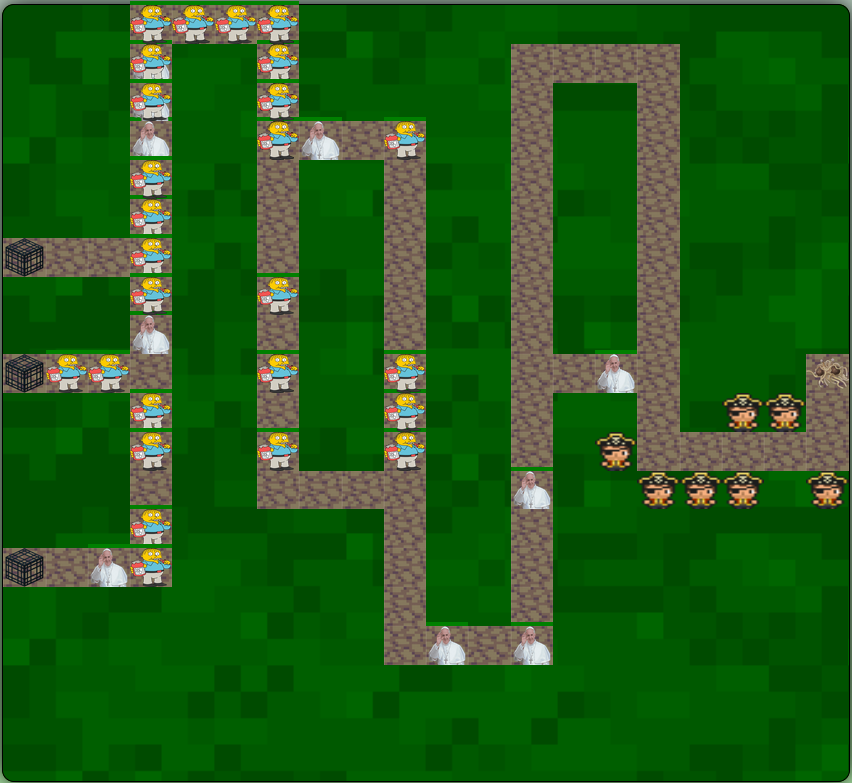
\includegraphics[height=6cm]{pastafarist_20.png} }}%   
    \caption{Différents affichages du jeu réalisé.}%
    \label{fig:affichages}%
     \vspace*{-0.3cm}
\end{figure}

\section{Réalisation}

Cette partie concerne des implémentations particulièrement intéressantes répondant aux besoins énoncés dans la \hyperref[sec:conception]{section \ref{sec:conception}}. Une première problématique à résoudre était la génération de chemin dans le jeu, que nous avons décidé 

\subsection{Génération aléatoire de chemin}
Nous résolvons le problème de génération aléatoire de chemin en deux étapes. D'abord, nous positionnons des points de passage, ensuite nous les connectons pour former le chemin final.

\subsubsection{Génération des points de passage}
Un point de passage est une position par laquelle le chemin généré doit passer.

Les points de passage sont générés en considérant une direction à prendre le long d'un axe du monde. Par exemple, il peuvent être générés de manière à ce que chaque nouveau point de passage ait une coordonnée supérieure sur l'axe des abscisses au point de passage précédent.
Les premiers points de passage se situent sur les acteurs de type Spawner, et les derniers points de passages sur les acteurs de type Spaghetti Monster.\\
Pour que les chemins ne soient jamais trop courts, nous contraignons les spawners à être générés sur un bord du plateau de jeu opposé au bord sur lequel seront générés les monstres en spaghetti.
Les spawners sont donc répartis sur un axe (qu'on appellera "axe des spawners") dont la direction est perpendiculaire à la direction selon laquelle les points de passages sont générés. Les points de passage sont numérotés dans l'ordre croissant en fonction de leur coordonnée sur l'axe perpendiculaire à l'axe des spawners. Cette numérotation définit l'ordre dans lequel ils doivent être parcourus, comme le présente la \hyperref[fig:points de passage]{Figure \ref{fig:points de passage}}.

\begin{figure}[H]
    \centering
    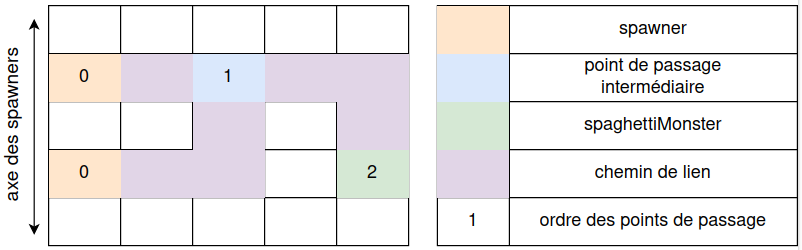
\includegraphics[width = 0.9\textwidth]{points_de_passage.png}
    \caption{Exemple de génération aléatoire de chemin dans un monde de taille 5 x 5.}
    \label{fig:points de passage}
\end{figure}

Il reste maintenant à lier ces points de passage pour former un ou plusieurs chemins menant des spawners aux monstres en spaghetti.

\subsubsection{Liaison des points de passage}

Nous voyons dans la \hyperref[fig:points de passage]{Figure \ref{fig:points de passage}} que des chemins de lien ont été générés. Ces chemins sont générés d'une manière très simple qui consiste à relier chaque point de passage de numérotation $n$ aux points de passage de numérotation $n - 1$, en commençant par placer des cases de chemin le long d'un axe (ici des abscisses) puis le long de l'autre axe (ici des ordonnées). La fonction reliant deux points de passage est une fonction récursive terminale prenant en paramètres une position initiale et une position finale à relier. À chaque appel récursif, il suffit de modifier la position initiale en l'ayant déplacé de une case vers la case finale, et ce jusqu'à ce que la case initiale corresponde à la case finale.

Il est facile de se convaincre que de cette manière, n'importe quel chemin peut être généré, pour peu qu'on place correctement les points de passage nécessaires à sa génération.
Pour une défense optimale, le joueur a tout intérêt à placer ses défenseurs autour de ce chemin.

\subsection{Joueur automatique}

Généralement, dans un jeu de Tower Defense, la répartition des défenseurs dans le monde est confiée au joueur. Jouer un coup consiste à placer un défenseur à une position donnée. Dans le cas du développement de notre jeu, ce placement est automatique et peu donc être vu comme faisant partie de la phase de spawn. Nous séparons tout de même ces deux phases dans un soucis de modularité.
Le joueur automatique est implémenté comme étant un acteur de type "player", possédant une action "play".

\subsubsection{Joueur intelligent}

Le joueur que nous avons implémenté diversifie ses coups à l'aide de deux algorithmes.
L'algorithme utilisé en priorité consiste à jouer des coups aléatoires proches des cases de chemin, en priorisant celles qui sont le moins nombreuses dans leur rangée. Une rangée étant dans la même direction que l'axe des spawners.

\begin{figure}[H]
    \centering
    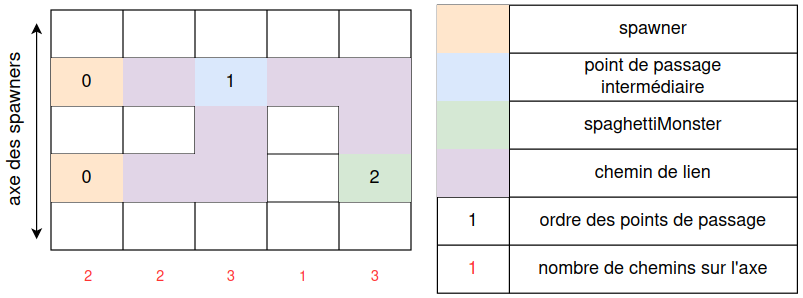
\includegraphics[width = 0.9\textwidth]{points_de_passage_play.png}
    \caption{Exemple de cases de chemin par rangéee dans un monde de taille 5 x 5.}
    \label{fig:points de passage play}
\end{figure}

Dans l'exemple de la \hyperref[fig:points de passage play]{Figure \ref{fig:points de passage play}}, les coups seront d'abord joués dans la 4ème rangée, puis dans les deux premières, et enfin dans les rangées 3 et 5.
Cet algorithme utilise un générateur de nombre aléatoires basé sur une implémentation pure récursive terminale du \hyperlink{https://fr.wikipedia.org/wiki/Mélange_de_Fisher-Yates}{mélange de Fisher-Yates}, qui termine.

L'implémentation de cet algorithme nous permet de passer en paramètres une portée dans laquelle les coups peuvent être joués, autour des cases.
Une fonction de distance, permettant de vérifier si la portée est respectée, doit également être précisée. Par exemple, la distance euclidienne peut être utilisée, et fournirait une portée circulaire.

Lorsque ce premier algorithme a épuisé ses possibilités, le joueur se met à jouer des coups valides aléatoires.

\subsubsection{Joueur aléatoire}

Ce deuxième algorithme énumère les positions libres, les mélange en utilisant la même implémentation du \hyperlink{https://fr.wikipedia.org/wiki/Mélange_de_Fisher-Yates}{mélange de Fisher-Yates}, et les parcourt jusqu'à trouver une position libre sur laquelle il peut jouer.

Il est évidemment possible d'utiliser ces deux algorithmes indépendamment, pour créer des joueurs aux comportements diversifiés. L'implémentation du joueur intelligent pourrait alors être légèrement amméliorée afin d'augmenter progressivement sa portée et finir par atteindre toutes les cases du plateau.

Une autre manière de créer des joueurs aux comportements diversifiés est d'utiliser le concept de décorateur fonctionnel.


\subsection{Diversification dynamique des comportements}

En exécutant le jeu, vous remarquerez que les attaquants ne se déplacent pas tous à la même vitesse. Et pourtant, ils utilisent tous la même fonction de déplacement! Le comportement de celle-ci est "simplement" augmenté en utilisant le principe de décorateur fonctionnel.  

\subsubsection{Choix d'implémentation des décorateurs, ou générateurs d'action}

Nos décorateurs fonctionnel \textbf{purs} permettent, de manière définitive comme dynamique, de modifier les comportements des entitées du jeu.
Ils permettent de ne pas avoir à écrire une nouvelle fonction, ou à passer de nombreux paramètres supplémentaires à toutes les fonctions de comportement, à chaque fois que l'on souhaite modifier un comportement.

En excluant les implémentations qui ne respectent pas le principe de pureté, au moins deux possibilités d'implémentation de ces décorateurs demeurent :
\begin{itemize}
    \item Modifier le type de retour des actions (une action décrivant un comportement) afin qu'elles retournent, en plus de leur résultat, la prochaine fonction à utiliser pour cette même action. Cette implémentation complexifie la création des actions, et rend leur type de retour beaucoup moins évident. Ce n'est pas la solution retenue. \label{text:decorateur1}
    \item Séparer les actions des \textbf{générateurs d'action}, qui seront utilisés pour mettre à jour les actions après les avoir exécutées. Dans cette implémentation, les actions restent inchangées, mais une nouvelle variable s'ajoute au type Actor, qui est un objet contenant pour chaque action son générateur, qui est une fonction retournant la prochaine action à utiliser, ainsi que le nouveau générateur, à l'état potentiellement différent, qui sera utilisé une fois la prochaine action exécutée. C'est la solution retenue.
\end{itemize}

Pour ralentir le déplacement d'un attaquant, il suffit de décorer son action de déplacement afin qu'elle ne soit éxecutée qu'une fois sur deux lorsqu'elle est appelée.

\subsubsection{Exemple concret}

En suivant le principe de généricité et de citoyenneté de première classe, nous avons programmé un décorateur \ref{fig:deco_every_n} qui prend en paramètres une fonction à décorer, la fonction à exécuter lorsque la fonction décorée ne doit pas être appelée, et une valeur définissant tous les combien de tours la fonction décorée doit être exécutée. On peut se servir des actions par défaut déjà programmées, telles que le déplacement de 0 case, qui revient à ne pas se déplacer, pour définir la fonction par défaut.
Ce décorateur retourne l'exécution d'une fonction interne, qui est un générateur d'action, en suivant le principe de fermeture. Ce générateur d'action retourne l'appel \textbf{gelé} d'un autre générateur, dont les paramètres auront été mis à jour, et l'action générée, qui définira le prochain comportement de l'entité concernée. Le gel du générateur retourné permet d'éviter un appel récursif infini. Cette fonction est typée de manière récursive, et un type ActionGenerators décrivant les générateurs d'action qu'un acteur doit contenir est créé, et basé sur le type ActorActions qui définissait déjà les types des actions des acteurs.


\begin{figure}[H]
    \centering
    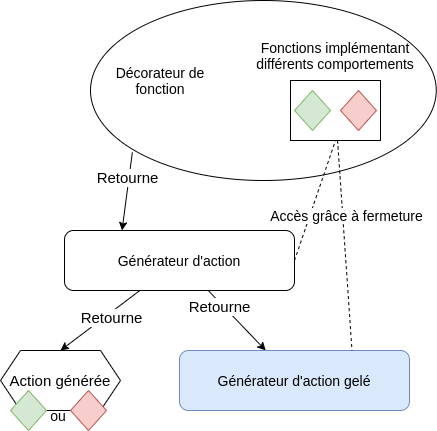
\includegraphics[width = 0.5\textwidth]{diag_deco_every_n.png}
    \caption{Décomposition d'un décorateur retournant alternativement une des fonctions données.}
    \label{fig:deco_every_n}
\end{figure}

\subsubsection{Mise à jour des actions et des générateurs}

Pour que cette implémentation fonctionne, il faut que le générateur et l'action soient mis à jour à chaque exécution de l'action. Ceci n'est pas automatiquement réalisé par l'action, et c'est le système de \textbf{phases} qui nous permet de mettre en place et synchroniser cette mise à jour.
Les phases permettent de mettre à jour les acteurs en fonction de leurs intentions. Cela suppose que l'action de l'acteur concernant la phase en question, de déplacement par exemple, a été exécutée et a donné son résultat. La fonction d'éxécution propre à la phase, et retournant le nouvel acteur en prenant en compte les intentions retournées par l'action de l'acteur, en profite donc pour retourner un acteur dont le générateur et l'action on tous les deux été mis à jour.

\subsubsection{Pour aller plus loin}

En suivant cette implémentation des phases et des générateurs d'action, un acteur n'est pas le seul à pouvoir modifier son propre comportement. N'importe quelle phase pourrait traîter les données qu'elle reçoit de manière à ce qu'un acteur modifie le comportement d'un autre acteur. Par exemple, les défenseurs pourraient ralentir les attaquants, en précisant dans le retour de leur action, le décorateur devant être utilisé sur les actions des attaquants affectés.
On pourrait imaginer d'autres scénarios qui complexifient légèrement le programme : la décoration des décorateurs. En effet, un attaquant pourrait grâce à un décorateur ne se déplacer qu'une fois tous les deux tours. Un défenseur paralyse cet attaquand pendant 3 tours, qui ne peut alors pas se déplacer. L'action décorée doit donc être encore décorée. On doit donc pouvoir créer plusieurs niveaux de décoration, et dans notre implémentation, il faudrait alors pouvoir décorer non pas l'action, mais le générateur d'actions. Cela n'a pas été implémenté, mais nous immaginons qu'il faudrait alors que les générateurs d'action retournent :
\begin{itemize}
    \item Le prochain générateur d'actions 'parent' à appeler.
    \item L'état du générateur d'action imbriqué (qui peut aussi être retourné comme générateur d'action 'parent' lorsque le générateur d'action 'parent' effectue sa dernière exécution).
    \item L'action générée (sur plusieurs niveaux de décoration, cette action correspondrait à la fonction par défaut du générateur 'parent' ou le résultat du générateur imbriquée, dont l'état devra alors être mis à jour).
\end{itemize}

Cette structuration permettrait plusieurs niveaux de décoration.

\section{conclusion}

Les efforts de pureté et modularité effectués dans ce projet nous permettent de facilement tester et maintenir chaque fonction, sans toujours devoir créer tout un environnement d'exécution pour celles-ci, et sans se préoccuper des changements de l'état de l'environnement.

Les inconvénients sont parfois la complexification d'écriture des fonctions, notamment des décorateurs fonctionnels purs.

La pureté n'est pas compatible avec l'aléatoire. On pourrait argumenter sur le fait que l'aléatoire n'existe pas et qu'on est sur un système pseudo-aléatoire. Cependant, une vrai piste d'ammélioration vers plus de pureté serait plutôt que les fonctions se servant de l'aléatoire prennent en paramètre cette fonction aléatoire, ou bien même directement son résultat. On pourrait alors tester ces fonctions de manière précise et exhaustive.

Les inconvénients du paradigme de programmation utilisé comprennent également les réductions de performance, notre programme ne souffre cependant pas de ce problème. De plus, dans un jeu du type tower defense, le délais entre les tours de jeu combiné à de la programmation asynchrone peut permettre de rendre ce problème invisible.

\end{document}